\section{测量合同与补充细节}

\subsection{C63 seed provenance}
质量评估在所报告的 NFE 下始终使用相同的三个配对训练 seed：20260891、20260892 和 20260893。完整逐 seed 测量值与分析文件已放在公开 GitHub 仓库中。

\paragraph{测量层级。}
E1 在双边际验证器通过之后，结束于实测 coupling 输出或势函数。E2 包含固定下游消费者。E3 包含训练、生成或任务评估。C82、C66 与 C80 记录 E2 端点，C63 记录 E3 训练端点。正文 C82 比率直接使用其登记的 E2 端点。C66 与 C80 在形成比率和 bootstrap 之前，先从每个单元中减去配对消费者时间；C63 使用记录的 solver 字段。EXP-PACKER19 为每个停止控制器和执行模式单元直接记录 E1。E2/E3 中不变的消费者或模型时间会稀释对应的 OT 阶段收益。C63 的固定宽度/动态压缩内部训练消融比率由完整 fixed-update E3 区间计算。

\paragraph{GPU 能耗区间。}
GPU 能耗取 A100 NVML 累计总能耗 counter 在已登记方法调用之前与最终 CUDA synchronization 之后的差值。Counter 以毫焦耳报告，分析将差值换算为焦耳。该 ready-arrays-to-consumer 区间包含 solver/proposal 与 consumer 工作，并排除编译、warm-up 和 prepared-input transfer 组件。不支持该 counter 时，记录为 unavailable，不使用功率上限估计替代。

\paragraph{C82 匹配固定宽度/动态压缩对照。}
C82 在相同的 MetroPT-3 failure-3 输入、冷启动 proposal、正则化、容差、验证检查时点、双边际验证器、packed backend 和固定消费者上运行固定宽度路径与动态压缩路径。实验变量是通过验证器的 lane 是否从后续 kernel 中动态移除。一台主机提供四个彼此独立的完整设备 A100 worker，不使用 worker 间 collective 或问题切分。对于每个 plan 和计时重复，端点取四个 worker 的 ready-arrays-to-consumer 最大时间。每个 plan 对两次计时重复取中位数，报告的 $1.745535\times$ 是三个 plan 比率的描述性几何均值。plan 标识只冻结执行顺序，不是独立 MetroPT 样本。48 个 worker-level repeat 全部收敛；最大行、列 $L_1$ 残差分别为 $9.476650\times10^{-4}$ 和 $1.283915\times10^{-6}$。在冻结消费者下，两臂的 failure-window ROC AUC 都为 $1.0$，求解器不使用标签。最大配对 transport-cost 与 barycentric-shift 差分别为 $0.02792263$ 和 $0.00346756$。

\paragraph{C66 双主机匹配对照。}
在 C66 的匹配对照中，固定宽度路径与动态压缩路径使用相同输入、冷启动 proposal、正则化、容差、验证检查时点、双边际验证器、packed backend 和固定消费者；根据停止规则释放问题与动态压缩是受控差异。三个顺序平衡的 plan 会在两台主机各自的四个 GPU placement 上复用。GPU placement 与 timing repeat 用于稳定端到端测量；登记的端点比率包含不变的非 OT 消费者时间。正文 C66 OT 阶段比率在每个 host--plan 单元内部减去配对消费者时间。host--plan 组合是该冻结 workload 的配对计时单元；placement 和 repeat 是 timing replica，而非独立 MetroPT workload。对六个有效 host--plan 单元的重分析报告分层 bootstrap 区间。

\paragraph{EXP-PACKER19 来源。}
停止--执行协议的 SHA-256 为 \nolinkurl{c010bcf9b3e276c8269514324cc8ed4bc2fc5958c362c7b880e3946dee75075b}，并绑定 source commit \nolinkurl{96de52b8ceff8fa3c0468bf45567e6b017483e73}。两台主机、每台四张 A100-SXM4-80GB GPU、三种冻结方法顺序和三次 timing repeat 产生 768 个正式单元。每个容差具有 24 个配对的 host--order--GPU 单元和 equal-host bootstrap 区间。Consumer TV 用于数值检查输出差异。

\begin{figure}[t]
\centering
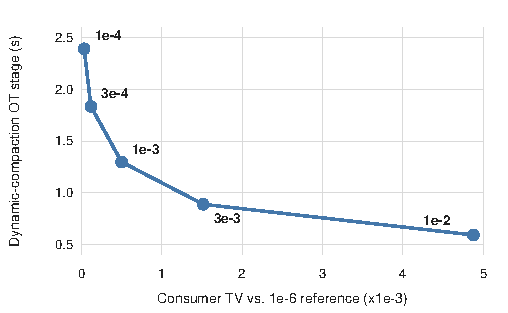
\includegraphics[width=\columnwidth]{../forgetting_ot_e2e_closure/figures/PACKER19_PARETO.pdf}
\caption{Packer19 随容差变化的 OT 速度--输出前沿，使用 dynamic-compaction 路径。每个点是在该残差容差下 24 个配对单元的 E1 OT 阶段时间中位数；consumer TV 相对本实验的 $10^{-6}$ 紧参考测量。}
\label{fig:packer-pareto}
\end{figure}

\paragraph{执行模式协议。}
正式实验在计时前固定 representation、width、execution mode、检查间隔、stopping tolerance、checking path、窄尾 handoff 阈值与 fail-closed 策略。宽度与分组干预映射选择固定宽度执行或动态压缩的条件。

\paragraph{宽度成本诊断来源。}
原语扫描使用一张具有 108 个 SM 的 NVIDIA A100-SXM4-80GB，driver 为 535.129.03，PyTorch 2.5.1 配 CUDA 12.4，Triton 3.1.0，source commit 为 \nolinkurl{73aec2941bfa1a5caa6a6bddf7aa83b734f9bb8b}。每次实测 \texttt{shifted\_step} 调用包含两个 packed Triton log-sum-exp kernel，并排除边缘 screen、双边际验证器、动态压缩与 \texttt{solve\_batch} 外层循环。Warm-up 后，width 在 30 次 repeat block 内随机化。$n=1024$ 扫描 width 1--8、10、12 与 16；$n=4096$ 和 $n=16384$ 扫描 1、2、3、4、6、8、12 与 16。该诊断提供式 \eqref{eq:time-difference} 中实测宽度成本曲线的 packed-update 组成部分。

\paragraph{独立后端实现。}
OTT-JAX 与 PyKeOps 路径通过各自原生后端机制移除已完成问题。OTT-JAX 执行固定的 20-update phase，在 phase boundary 检查，移除通过 lane，并对存活问题重新分桶；原生 \texttt{vmap} 和匹配的 fixed-phase static 路径作为对照。PyKeOps 路径使用一个独立问题批量 matrix-free operator、固定几何验证检查时点、双边际验证器，以及对通过问题状态的动态移除。Sequential 与 static-padded PyKeOps 路径使用相同 symbolic backend。共享原理是逐问题释放并动态移除已完成项；检查和 packing 机制仍由后端决定。\Cref{tab:ot-cross-backend} 中所有跨后端结果都报告实际达到的两侧边缘残差。

\subsection{独立后端实现}

\begin{table*}[t]
\centering
\caption{OTT-JAX 与 PyKeOps 在真实数据上的独立实现。每个比率均为基线时间除以压缩路径时间；不确定性标签分别说明 timing-repeat range 或 observed-input range。}
\label{tab:ot-cross-backend}
\scriptsize
\setlength{\tabcolsep}{3.0pt}
\resizebox{\textwidth}{!}{%
\begin{tabular}{@{}llllll@{}}
\toprule
后端 & Workload & OT 阶段对照 & 加速比（不确定性） & 计时；单元 & 精度合同 \\
\midrule
OTT-JAX & ImageNet-32, $n=4096,W=16$ & native vmap / 每个固定阶段处理剩余问题 & \COTTNativeActiveSpeedup{} (repeat range \COTTNativeActiveRange{}) & direct E1; 6 timing repeats & max L1 $9.97\!\times\!10^{-4}$ \\
PyKeOps & A2D2 LiDAR, $n=8192,W=8$ & sequential carry / active & \CKeopsLiDARActiveSpeedup{} (clip range \CKeopsLiDARActiveRange{}) & direct E1; 3 real clips & max L1 $9.97\!\times\!10^{-4}$ \\
PyKeOps & ImageNet-32, $n=16384,W=4$ & sequential / active & \CKeopsImageNetActiveSpeedup{} (seed range \CKeopsImageNetActiveRange{}) & direct E1; 3 seeds & max L1 $8.93\!\times\!10^{-4}$ \\
\bottomrule
\end{tabular}}
\end{table*}


\begin{table}[t]
\centering
\caption{主要正式 workload 配置。各行均使用冷启动，以及检查当前两侧边缘残差的验证器。}
\label{tab:workload-configs}
\scriptsize
\setlength{\tabcolsep}{3pt}
\begin{tabular}{@{}p{.16\columnwidth}p{.76\columnwidth}@{}}
\toprule
实验 & 端点、数值配置与统计单元 \\
\midrule
C82 & MetroPT-3 预测性维护 (E2)；$(n,W,\varepsilon)=(16{,}384,16,.1)$；检查间隔 4；$\tau=10^{-3}$；一台主机、四个完整设备 worker、三个顺序 plan、两次计时重复。 \\
C66 & MetroPT-3 预测性维护 (E2)；$(n,W,\varepsilon)=(16{,}384,16,.1)$；检查间隔 4；$\tau=10^{-3}$；两台主机、三个 plan。 \\
C80/LM & Packer19 scRNA 转移 (E2)；$(16{,}384,8,.1)$；检查间隔 4；$\tau=10^{-3}$；24 个配对单元。 \\
EXP-P19 & Packer19 同控制器 Pareto (E1)；$(16{,}384,8,.1)$；检查间隔 4；$\tau=10^{-4}\text{--}10^{-2}$；每个容差 24 个配对单元。 \\
C63 & ImageNet-32 PCA500 OT-FM (E3)；$(1{,}024,8,.03)$；检查间隔 4；$\tau=10^{-3}$；三个配对 seed。 \\
\bottomrule
\end{tabular}
\end{table}


\section{部署与运行边界}

\paragraph{完整设备执行与按行划分矩阵。}
当一个问题能放入一个加速器时，完整设备 worker 处理不同窗口，不需要 Sinkhorn collective。按行划分矩阵为单个超大问题提供容量路径。完整设备执行是 C67 使用的 throughput 路径。在一台主机上，从一个 worker 增加到四个 worker，会在两条 held-out MetroPT route 上产生 $3.965$--$3.979\times$ fixed-per-worker throughput scaling。双主机八 worker fixed-per-worker 实验报告该 worker 数下的端点比较。本文把 one-to-four 与双主机八 worker 作为两个独立 scaling study 报告。峰值内存保持为每个 worker 的本地内存。

\subsection{补充归因与证据边界}
\begin{table*}[t]
\centering
\caption{三个 packed-Triton workload 在 $10^{-3}$ 工作点的绝对 OT 阶段时间（秒）。Packer19 报告 24 个配对 host--order--GPU 单元的中位数；ImageNet-32 报告三个配对训练 seed 上 solver 阶段的均值 $\pm$ 样本标准差；MetroPT-3 报告三个已登记 worker-1 plan 单元的中位数。Packer19 不报告固定宽度值，因为其已登记固定宽度实验臂实际执行了 compaction 分支，故予以排除。破折号表示没有可用的匹配实验臂。配对效应另行报告。}
\label{tab:absolute-ot-times}
\small
\resizebox{\textwidth}{!}{%
\begin{tabular}{@{}lccc@{}}
\toprule
Workload & 固定宽度批次 & 逻辑 mask & 动态压缩\\
\midrule
Packer19 (EXP-P19; $n=16384,W=8$) & --- & 2.038 & 1.299 \\
MetroPT-3 (C66; $n=16384,W=16$) & 14.839 & --- & 8.462 \\
ImageNet-32 PCA500 (C63) & $122.17\pm2.91$ & --- & $115.89\pm0.83$ \\
\bottomrule
\end{tabular}}
\end{table*}

\begin{table*}[t]
\centering
\caption{所报告归因对照的证据索引。比率均为分子路径时间/分母路径时间；大于 1 表示分母更快。GM 为几何均值。各实验的计时范围及样本/重复单元逐行列出。C33 是较早项目 adapter 的受控重叠 support 实验。C62/C63 的正则化参数为 0.03，其余各行为 0.1。完整实验目录及排除记录见来源总账。}
\label{tab:attribution-map}
\scriptsize
\setlength{\tabcolsep}{2pt}
\begin{tabular}{@{}>{\raggedright\arraybackslash}p{.068\textwidth}>{\raggedright\arraybackslash}p{.14\textwidth}>{\raggedright\arraybackslash}p{.133\textwidth}>{\raggedright\arraybackslash}p{.070\textwidth}>{\raggedright\arraybackslash}p{.090\textwidth}>{\raggedright\arraybackslash}p{.095\textwidth}>{\raggedright\arraybackslash}p{.17\textwidth}>{\raggedright\arraybackslash}p{.15\textwidth}@{}}
\toprule
实验 & 后端 / workload & $n,W;\tau$ & Proposal & 对照 & 比率 & 计时范围 & 样本 / 重复 \\
\midrule
C82 & packed Triton / MetroPT-3 & $16384,16;10^{-3}$ & 冷启动 & fixed/\allowbreak dynamic & 1.745535 & E2 四 worker makespan；slots $5696/3128=1.820972\times$ & plans 1.745273 / 1.745356 / 1.745975；2 次重复 \\
C66 & packed Triton / MetroPT-3 & $16384,16;10^{-3}$ & 冷启动 & fixed/\allowbreak dynamic & 1.754 & OT 阶段；逐对扣除 consumer & host--plan 单元 \\
C63 & packed Triton / ImageNet-32 & $1024,8;10^{-3}$ & 冷启动 & fixed/\allowbreak dynamic & 1.054 & solver 字段；补充 GM & 3 个训练 seed \\
C63 & packed Triton / ImageNet-32 & $1024,8;10^{-3}$ & 冷启动 & fixed/\allowbreak dynamic & 1.036 & 完整固定步数训练 & 3 个训练 seed \\
C62 & packed Triton / ImageNet-32 & $1024,8;10^{-3}$ & 冷启动 & fixed/\allowbreak dynamic & 1.105 & coupling 准备 & 3 个 problem-plan seed \\
C67 & packed Triton / MetroPT routes 2,3 & $16384,8;10^{-3}$ & 冷启动 & fixed/\allowbreak dynamic & 3.110 / 2.159 & 8-worker 端点；每 worker 工作量固定 & 2 条路线；host/plan 重复 \\
C67 & packed Triton / MetroPT route 3 & $8192,16;10^{-3}$ & 冷启动 & fixed/\allowbreak dynamic & 2.316 & 单 worker 端点；等主机 GM & 2 台主机；各 3 个 plan \\
C67 & packed Triton / MetroPT route 3 & $32768,16;10^{-3}$ & 冷启动 & fixed/\allowbreak dynamic & 1.616 & 单 worker 端点；等主机 GM & 2 台主机；各 3 个 plan \\
C55 & OTT-JAX / ImageNet-32 & $4096,16;10^{-3}$ & 固定 & fixed/\allowbreak dynamic & 1.581 & 匹配 20-update 阶段 & 一个输入；10 次重复 \\
C55 & OTT-JAX / ImageNet-32 & $4096,16;3\!\times\!10^{-3}$ & 固定 & fixed/\allowbreak dynamic & 1.556 & 匹配 10-update 阶段 & 一个输入；10 次重复 \\
C55 & OTT-JAX / ImageNet-32 & $4096,16;5\!\times\!10^{-3}$ & 固定 & fixed/\allowbreak dynamic & 1.366 & 匹配 10-update 阶段 & 一个输入；10 次重复 \\
C55 & OTT-JAX / ImageNet-32 & $4096,16;10^{-2}$ & 固定 & fixed/\allowbreak dynamic & 0.995 & 匹配 10-update 阶段 & 一个输入；10 次重复 \\
C33 & packed Triton / ImageNet-32 & $4096,16;10^{-3}$ & 共享 anchor & fixed/\allowbreak dynamic & 1.421 & steady-state 关键路径 & 40 个受控窗口 \\
C80-LM & packed Triton / Packer19 & $16384,8;10^{-3}$ & 冷启动 & fixed/LM & 1.000 & OT 阶段；逐对扣除 consumer & 24 个 host--order--GPU 单元 \\
C80-LM & packed Triton / Packer19 & $16384,8;10^{-3}$ & 冷启动 & LM/DC & 1.540 & OT 阶段；逐对扣除 consumer & 24 个 host--order--GPU 单元 \\
EXP-P19 & packed Triton / Packer19 & $16384,8;10^{-4}$--$3\!\times\!10^{-3}$ & 冷启动 & LM/DC & 1.480--1.638 & 直接 OT 阶段；四个容差 & 每容差 24 个配对单元 \\
EXP-P19 & packed Triton / Packer19 & $16384,8;10^{-2}$ & 冷启动 & LM/DC & 0.9995 & 直接 OT 阶段；同步释放 & 每容差 24 个配对单元 \\
\bottomrule
\end{tabular}
\end{table*}

\begin{table}[t]
\centering
\caption{逐 seed 的 C63 solver 时间（秒）及固定宽度/动态压缩。对已有记录进行描述性配对重分析；三个比值的几何均值为 $1.054$。}
\label{tab:c63-solver-pairs}
\small
\begin{tabular}{@{}rrrr@{}}
\toprule
Seed & 固定宽度 (s) & 动态压缩(s) & 固定/动态 \\
\midrule
20260891 & 123.429 & 116.699 & 1.058 \\
20260892 & 124.233 & 115.934 & 1.072 \\
20260893 & 118.840 & 115.036 & 1.033 \\
\bottomrule
\end{tabular}
\end{table}

\begin{table}[t]
\centering
\caption{C80-LM 阶段时间（秒）：匹配实现中各组件的边际中位数。各阶段分别汇总；总时间比率由配对的完整路径计时计算，见 \cref{tab:c80-attribution}。}
\label{tab:phase-costs}
\small
\begin{tabular}{@{}lrr@{}}
\toprule
阶段 & LM (s) & PC (s) \\
\midrule
修正 & 1.7063 & 1.0708 \\
验证检查 & 0.6385 & 0.4006 \\
Verifier & 0.1045 & 0.1045 \\
Mask / compaction & 0.000306 & 0.003370 \\
\bottomrule
\end{tabular}
\end{table}


C62 固定 packed Triton adapter、输入和数值合同，只改变动态压缩；三个固定宽度/动态压缩比值为 $1.156$、$1.082$ 和 $1.079$。固定宽度/动态压缩 slots 分别为 $64/52$、$64/56$ 和 $64/56$。这些测量覆盖 coupling 准备。C55 在每个容差上使用一个冻结 ImageNet-32 输入和十次计时重复；phase size 在独立 warmup bank 上选择。$10^{-2}$ 时的 $0.995\times$ 与匹配 phase 的正结果一起保留。

C67 的全局八 worker 结果在每个 worker 工作量固定的条件下汇总完整 consumer 端点。路线 2 的固定宽度/动态压缩秒数为 $12.523/4.026$，路线 3 为 $7.999/3.705$；实际执行 slots 分别为 $4736/1276$ 和 $3008/1244$。报告的 support-size 加速包括路线 3 上 $n=8192$ 与 $32768$ 两个在两台主机均通过冻结门的单元。连续 transport-cost 与 barycentric-shift 差异是在已登记二元 consumer 端点下报告的诊断量。

C33 的非冷启动结果在真实 ImageNet 特征上使用构造的 90\% overlap target stream。其 canonical 反序 warm replay 排除 compile、cache load 和进程启动，同时保留 descriptor、传输、anchor、proposal、correction 和 verification 成本。M3 的分组比值描述一个固定的 32 问题集合；oracle 迭代编号 $q_t$ 定义分组干预。固定集合使 $\sum_t q_t$ 不变，分组则改变跨窗口的 $\sum_w W q_{\max,w}$。这些比率报告由此产生的相对运行时间效应；每种分组下的绝对实验臂时间可进一步分离固定宽度与压缩路径的变化。
